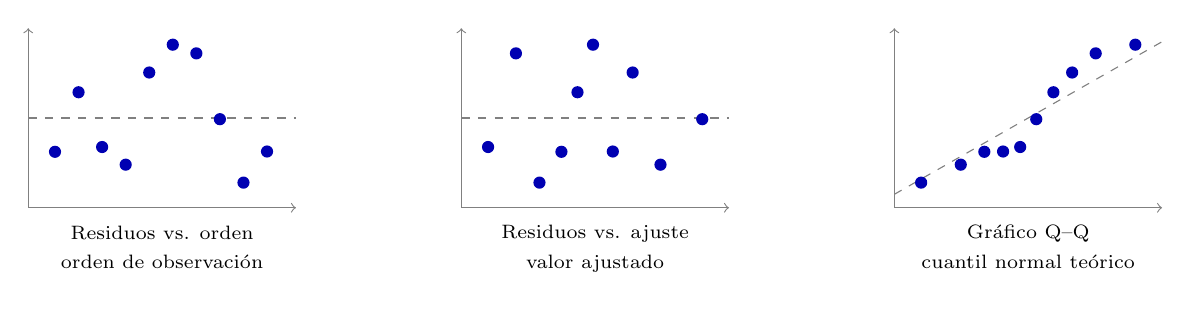
\begin{tikzpicture}[x=0.68cm,y=0.38cm,font=\scriptsize]
    % Residuos contra el orden de observación
    \begin{scope}
        \draw[->,gray] (0,-3) -- (5,-3);
        \draw[->,gray] (0,-3) -- (0,3);
        \draw[gray,dashed] (0,0) -- (5,0);
        \foreach \x/\e in {0.5/-1.13,0.94/0.86,1.38/-0.97,1.82/-1.56,2.26/1.52,2.70/2.45,3.14/2.16,3.58/-0.04,4.02/-2.16,4.46/-1.12} {\fill[blue!70!black] (\x,\e) circle (2.2pt);}
        \node[align=center] at (2.5,-3.85) {Residuos vs. orden};
        \node[below] at (2.5,-4.25) {orden de observación};
    \end{scope}
    % Residuos contra valores ajustados
    \begin{scope}[xshift=5.5cm]
        \draw[->,gray] (0,-3) -- (5,-3);
        \draw[->,gray] (0,-3) -- (0,3);
        \draw[gray,dashed] (0,0) -- (5,0);
        \foreach \x/\e in {1.87/-1.13,2.17/0.86,0.50/-0.97,3.72/-1.56,3.20/1.52,2.46/2.45,1.02/2.16,4.50/-0.04,1.46/-2.16,2.83/-1.12} {\fill[blue!70!black] (\x,\e) circle (2.2pt);}
        \node[align=center] at (2.5,-3.85) {Residuos vs. ajuste};
        \node[below] at (2.5,-4.25) {valor ajustado};
    \end{scope}
    % Gráfico Q--Q con los residuos ordenados
    \begin{scope}[xshift=11cm]
        \draw[->,gray] (0,-3) -- (5,-3);
        \draw[->,gray] (0,-3) -- (0,3);
        \draw[gray,dashed] (0,-2.55) -- (5,2.55);
        \foreach \x/\e in {0.50/-2.16,1.24/-1.56,1.68/-1.13,2.03/-1.12,2.35/-0.97,2.65/-0.04,2.97/0.86,3.32/1.52,3.76/2.16,4.50/2.45} {\fill[blue!70!black] (\x,\e) circle (2.2pt);}
        \node[align=center] at (2.5,-3.85) {Gráfico Q--Q};
        \node[below] at (2.5,-4.25) {cuantil normal teórico};
    \end{scope}
\end{tikzpicture}